\begin{enumerate}[label=\thechapter.\arabic*,ref=\thechapter.\theenumi]
\item Find the sum of the first $15$ multiples of $8$. \\

\solution
\iffalse
\let\negmedspace\undefined
\let\negthickspace\undefined
\documentclass[journal,12pt,twocolumn]{IEEEtran}
\usepackage{cite}
\usepackage{amsmath,amssymb,amsfonts,amsthm}
\usepackage{algorithmic}
\usepackage{graphicx}
\usepackage{textcomp}
\usepackage{xcolor}
\usepackage{txfonts}
\usepackage{listings}
\usepackage{enumitem}
\usepackage{mathtools}
\usepackage{gensymb}
\usepackage{comment}
\usepackage[breaklinks=true]{hyperref}
\usepackage{tkz-euclide} 
\usepackage{listings}
\usepackage{gvv}                                        
\def\inputGnumericTable{}                                 
\usepackage[latin1]{inputenc}                                
\usepackage{color}                                            
\usepackage{array}                                            
\usepackage{longtable}                                       
\usepackage{calc}                                             
\usepackage{multirow}                                         
\usepackage{hhline}                                           
\usepackage{ifthen}                                           
\usepackage{lscape}
\newtheorem{theorem}{Theorem}[section]
\newtheorem{problem}{Problem}
\newtheorem{proposition}{Proposition}[section]
\newtheorem{lemma}{Lemma}[section]
\newtheorem{corollary}[theorem]{Corollary}
\newtheorem{example}{Example}[section]
\newtheorem{definition}[problem]{Definition}
\newcommand{\BEQA}{\begin{eqnarray}}
\newcommand{\EEQA}{\end{eqnarray}}
\newcommand{\define}{\stackrel{\triangle}{=}}
\theoremstyle{remark}

\newtheorem{rem}{Remark}
\begin{document}
\parindent 0px
\bibliographystyle{IEEEtran}
\title{Assignment 10.5.3\_13Q}
\author{EE23BTECH11219 - Rada Sai Sujan$^{}$% <-this % stops a space
}
\maketitle
\newpage
\bigskip
\section*{Question}
Find the sum of the first $15$ multiples of $8$. \\
\solution
\fi

\begin{table}[ht]
    \centering
    \def\arraystretch{1.5}
    \begin{tabular}{|p{2cm}|p{2.5cm}|p{2.3cm}|}
    \hline
    PARAMETER & VALUE & DESCRIPTION  \\ \hline
    $$x\brak0$$ & $$8$$ & First term \\ \hline
    $$d$$ & $$8$$ & common difference \\ \hline
    $$x(n)$$ & $$[8+8n]u\brak n$$ & General term of the series  \\ 
    \hline
  \end{tabular}

    \caption{Parameter Table1}
    \label{tab:10.5.3.1}
\end{table}
For an $AP$,
\begin{align}
    X\brak z &= \frac{ x\brak 0 }{1-z^{-1}} + \frac{dz^{-1}}{{(1-z^{-1})}^{2}}    \\
    \implies X\brak z &= \frac{8}{1-z^{-1}} + \frac{8z^{-1}}{{(1-z^{-1})}^{2}} \\
    &= \frac{8}{({1-z^{-1})}^{2}} ,\quad \abs{z}>1    \\
    y\brak{n}&=x\brak{n}\ast u\brak{n}\\
    \implies Y\brak{z}&=X\brak{z}U\brak{z}   \\
    Y\brak{z}&=\brak{\frac{8}{({1-z^{-1})}^{2}}}\brak{\frac{1}{1-z^{-1}}}  \\
    &=\frac{8}{({1-z^{-1})}^{3}} ,\quad \abs{z}>1 
\end{align}
 Using Contour Integration to find the inverse $Z$-transform,
\begin{align}
    y(14)&=\frac{1}{2\pi j}\oint_{C}Y(z) \;z^{13} \;dz  \\
    &=\frac{1}{2\pi j}\oint_{C}\frac{8z^{13}}{({1-z^{-1})}^{3}} \;dz 
\end{align}
We can observe that the pole is repeated $3$ times and thus $m=3$,
\begin{align}
    R&=\frac{1}{\brak {m-1}!}\lim\limits_{z\to a}\frac{d^{m-1}}{dz^{m-1}}\brak {{(z-a)}^{m}f\brak z}  \\
    &=\frac{1}{\brak {2}!}\lim\limits_{z\to 1}\frac{d^{2}}{dz^{2}}\brak {{(z-1)}^{3}\frac{8z^{16}}{{(z-1)}^3}}   \\
    &=4\lim\limits_{z\to 1}\frac{d^2}{dz^2}(z^{16})   \\
    &=960
\end{align}
\begin{align}
    \therefore \boxed{y(14)=960}
\end{align}
\begin{figure}[ht]
        \centering
        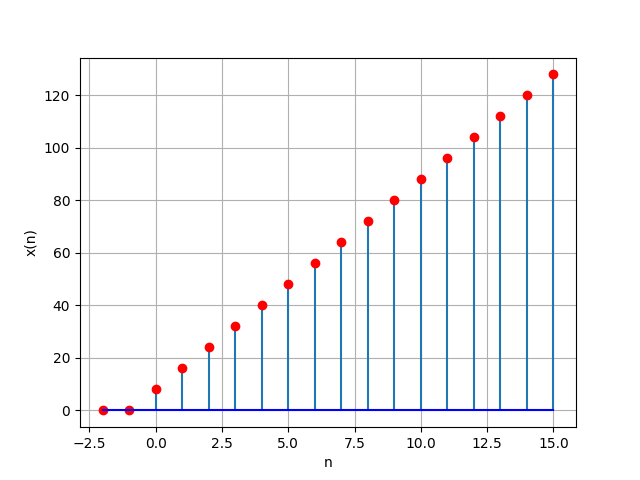
\includegraphics[width=\columnwidth]{ncert-maths/10/5/3/13/figs/a.png}
        \caption{Plot of x(n) $vs$ n}
        \label{fig:10.5.3.13.1}
    \end{figure}
    

%\pagebreak

\item If the sum of $n$ terms of an A.P. is $3n^2+5n$ and its $m^{th}$ term is 164, find the value of $m$.\\
\solution
\iffalse
\documentclass[journal,12pt,twocolumn]{IEEEtran}
\usepackage{amsmath,amssymb,amsfonts,amsthm}
\usepackage{txfonts}
\usepackage{tkz-euclide}
\usepackage{listings}
\usepackage{gvv}
\usepackage[latin1]{inputenc}
\usepackage{array}
\usepackage{pgf}
\usepackage{lmodern}

\begin{document}
\bibliographystyle{IEEEtran}

\vspace{3cm}

\title{}
\author{EE23BTECH11054 -  Sai Krishna Shanigarapu$^{*}$
}
\maketitle
\newpage
\bigskip



\section*{Exercise 9.2}

13. \hspace{2pt}If the sum of $n$ terms of an A.P. is $3n^2+5n$ and its $m^{th}$ term is 164, find the value of $m$.
\bigskip

\solution
\fi
\begin{align}
Y\brak{z} &=  \sum_{n=0}^{\infty} y\brak{n}z^{-n} \\
&= \frac{2\brak{4-z^{-1}}}{\brak{1-z^{-1}}^3}, \qquad |z| > 1\\
U\brak{z} &= \frac{1}{1-z^{-1}}, \qquad |z| > 1\\
X\brak{z} &=  \frac{Y\brak{z}}{U\brak{z}}\\
 &= 2\brak{\frac{1}{1-z^{-1}}} + 6\brak{\frac{1}{\brak{1-z^{-1}}^2} } \\
 &= \frac{8z^2 - 2z}{\brak{z-1}^2} 
\end{align}


Using Contour Integration to find the inverse Z-transform,
\begin{align}
   x\brak{n} &= \frac{1}{2\pi j}\oint_C X\brak{z}z^{n-1}dz\\
    &= \frac{1}{2\pi j}\oint_C \frac{\brak{8z^{n+1} - 2z^{n}}dz}{\brak{z-1}^2}\\
    &= \frac{1}{\brak{m-1}!}\lim_{z\to\ a}\frac{d^{m-1}}{dz^{m-1}}\brak{\brak{z-a}^m f\brak{z}}\\
    &= \lim_{z\to\ 1}\frac{d}{dz}\brak{\brak{z-1}^2 \frac{8z^{n+1} - 2z^n}{\brak{z-1}^2}}\\
    &= \lim_{z\to 1}\brak{8\brak{n+1}z^n - 2nz^{n-1}}\\
    \implies x\brak{n} &= \brak{6n+8}\brak{u\brak{n}}\\
    164 &= \brak{6m+8}\brak{u\brak{m}}\\
    \implies m &= 26
\end{align}

\setlength{\arrayrulewidth}{0.3mm}
\setlength{\tabcolsep}{15pt}
\renewcommand{\arraystretch}{1.4}

\begin{table}[ht]
\centering

\begin{tabular}{|c|c|}
\hline

Symbol & Remarks\\
\hline
$y\brak{n} =\brak{3n^2+11n+8}\brak{u\brak{n}}$ & Sum of $n$ terms  \\
\hline
$x(m-1)$ & $164$\\
\hline
$y\brak{n}$ & $x\brak{n} * u\brak{n}$\\
\hline

\end{tabular}
\vspace{0.25cm}
\caption{Parameters}
\label{tab:11.9.2.13.1}



\end{table}



\begin{figure}[htbp]
    \centering
    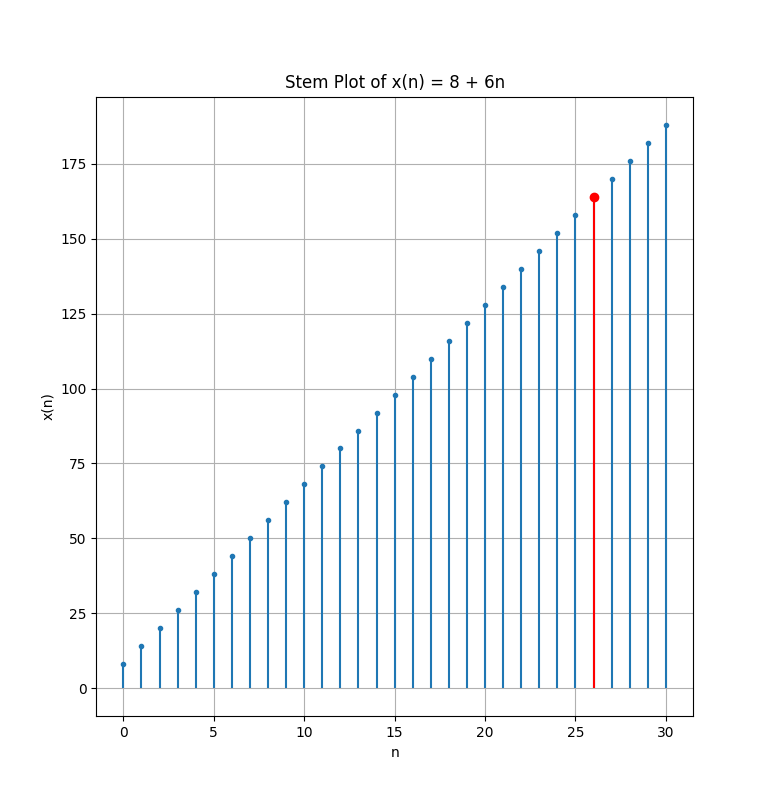
\includegraphics[width=1.0\columnwidth]{ncert-maths/11/9/2/13/figs/Figure_1.png}
    \caption{Plot of x(n) vs n}
    \label{fig:11.9.2.13.1}
\end{figure}


%\end{document}


\pagebreak
\item Find the sums given below:
\begin{enumerate}
    \item  $7 + \frac{21}{2} + 14 ... + 84$
    \item  $34 + 32 + 30 ... + 10$
    \item  $-5 + -8 + -11 ... -230$
\end{enumerate}
\solution
\iffalse
\let\negmedspace\undefined
\let\negthickspace\undefined
\documentclass[journal,12pt,onecolumn]{IEEEtran}
\usepackage{cite}
\usepackage{amsmath,amssymb,amsfonts,amsthm}
\usepackage{algorithmic}
\usepackage{graphicx}
\usepackage{textcomp}
\usepackage{xcolor}
\usepackage{txfonts}
\usepackage{listings}
\usepackage{enumitem}
\usepackage{mathtools}
\usepackage{gensymb}
\usepackage{comment}
\usepackage[breaklinks=true]{hyperref}
\usepackage{tkz-euclide} 
\usepackage{listings}
\usepackage{gvv}    
\usepackage{enumitem}
\usepackage{amsmath}
\def\inputGnumericTable{}                                 
\usepackage[latin1]{inputenc}                                
\usepackage{color}                                            
\usepackage{array}                                            
\usepackage{longtable}                                       
\usepackage{calc}                                             
\usepackage{multirow}                                         
\usepackage{hhline}                                           
\usepackage{ifthen}                                           
\usepackage{lscape}
\usepackage{tabularx}

\newtheorem{theorem}{Theorem}[section]
\newtheorem{problem}{Problem}
\newtheorem{proposition}{Proposition}[section]
\newtheorem{lemma}{Lemma}[section]
\newtheorem{corollary}[theorem]{Corollary}
\newtheorem{example}{Example}[section]
\newtheorem{definition}[problem]{Definition}
\newcommand{\BEQA}{\begin{eqnarray}}
\newcommand{\EEQA}{\end{eqnarray}}
\newcommand{\define}{\stackrel{\triangle}{=}}
\theoremstyle{remark}
\newtheorem{rem}{Remark}
\begin{document}
\bibliographystyle{IEEEtran}
\vspace{3cm}

\title{NCERT-discrete : 10.5.3 - 2}
\author{EE23BTECH11025 - Anantha Krishnan $^{}$% <-this % stops a space
}
\maketitle
\bigskip



\section{question}

Find the sums given below:
\begin{enumerate}
    \item  $7 + \frac{21}{2} + 14 ... + 84$
    \item  $34 + 32 + 30 ... + 10$
    \item  $-5 + -8 + -11 ... -230$
\end{enumerate}

 



\textbf{Solutions :}
\fi
\begin{table}[ht!]
\centering
\begin{tabular}{ |c|c|c| } 
 \hline
Symbols & Description & Values  \\
 \hline
$d_i$ & Common Difference for $i^{th}$ AP & 3.5 \\ \cline{3-3}
 & & -2 \\ \cline{3-3}
 & & -3 \\ 
\hline

  $x_i(n)$ & $n^{th}$ term for $i^{th}$ Sequence &  ($7$ +$\frac{7n}{2}$)$u_{(n)}$\\ \cline{3-3}
 & &  ($34$ - $2n$)$u_{(n)}$ \\ \cline{3-3}
 & &  ($-5$ +$-3n$)$u_{(n)}$ \\ 
\hline


  $x_i(0)$ & First term for $i^{th}$ AP & 7 \\ \cline{3-3}
 & & 34 \\ \cline{3-3}
 & & -5 \\ 
\hline
  
   \hline
\end{tabular}
\caption{Parameters , Descriptions And Values }
\label{table:ee25-tab1}
\end{table}




\begin{enumerate}
\item
$ 7 + \frac{21}{2} + 14 ... + 84$

\begin{align}
x_1\brak{n} &= \brak{x_1\brak{0} + nd_1}u_{\brak{n}}\\
\implies 84 &= 7+\frac{7n}{2}\\
\implies n &= 22
\end{align}

\begin{enumerate}    
\item 
z-Transform of $x_1\brak{n}$ :
Using $\eqref{eq:ztrans}$
\begin{align}
X_1(z)&= \frac{7z}{z-1} + \frac{7z}{{2\brak{z-1}}^{2}} \label{eq:ee25-4}
,\quad \abs {z}>\abs{1} 
\end{align}
\item
Z-Transform of $y_1\brak{n}$ :
\begin{align}
    y_1\brak{n} &= x_1\brak{n} * h\brak{n} \\
         h\brak{n} &= u\brak{n} \\
                 H\brak{z} &= \frac{z}{z-1} \label{eq:ee25-9}\\
    Y_1\brak{z} &= X_1\brak{z} * H\brak{z}\\
 &= \brak{\frac{7z}{z-1}+
\frac{7z}{2\brak{z-1}^{2}}}\brak{\frac{z}{z-1}}
,\quad \abs {z}>\abs{1}     
\end{align}
        \item
Inversion of $Y_1\brak{z}$ :
Using Contour Integration :
\begin{align}
y_1(22)&=\frac{1}{2\pi j}\oint_{C}Y(z) \;z^{21} \;dz\\  
\implies &=\frac{1}{2\pi j}\oint_{C}\brak{\frac{7z^{23}}{\brak{z-1}^2}+
       \frac{7z^{23}}{2\brak{z-1}^3}} \;dz\\
      R&=\frac{1}{\brak {m-1}!}\lim\limits_{z\to a}\frac{d^{m-1}}{dz^{m-1}}\brak {{(z-a)}^{m}f\brak z}\label{eq:ee25-r}  
\end{align}
    For $R_1$ , $m=2$ , where $m$ corresponds to number of repeated poles . 
\begin{align}
  R_1 &=\frac{1}{\brak {1}!}\lim\limits_{z\to 1}\frac{d}{dz}\brak {{(z-1)}^{2}\frac{7z^{23}}{{(z-1)}^2}}   \\
    &=7\lim\limits_{z\to 1}\frac{d}{dz}(z^{23})   \\
    &= 161
    \end{align}
    For $R_2$ , $m=3$ 
    \begin{align}
    R_2 &=\frac{1}{\brak {2}!}\lim\limits_{z\to 1}\frac{d^{2}}{dz^{2}}\brak {{(z-1)}^{3}\frac{\brak{7z^{13}}}{{2(z-1)}^3}}   \\
    &=\brak{\frac{7}{4}}\lim\limits_{z\to 1}\frac{d^2}{dz^2}(z^{23})   \\
    &= \frac{1771}{2}\\
    R_1 + R_2 &= \frac{2093}{2}\\
    \implies  y_1{(22)} &= \frac{2093}{2}
\end{align}
\end{enumerate}   

    \begin{figure}[H]
    \centering
\graphicspath{ {ncert-maths/10/5/3/2/figs/} }
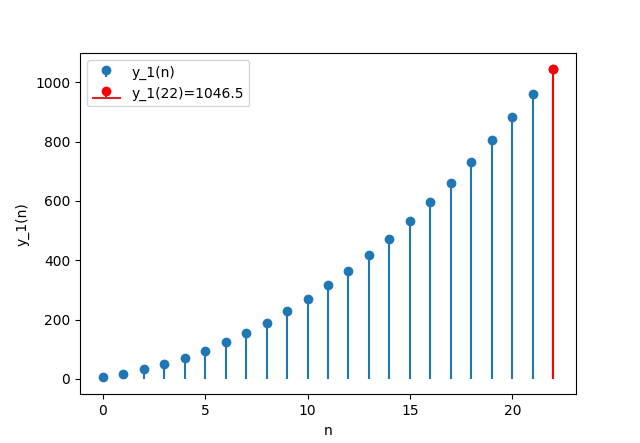
\includegraphics[width=\columnwidth]{graph_1}
\caption{ $y_1\brak{n}$ vs n }
\label{graph:ee25-g2}
\end{figure}




\item
 34 + 32 + 30 ... + 10


\begin{align}
x_2\brak{n} &= \brak{x_2\brak{0} + nd_2}u_{\brak{n}}\\
     \implies 10 &= 34 -2n\\
     \implies n &= 12 
     \end{align}

\begin{enumerate}
\item
Z-Transform of $x_2\brak{n}$ :
Using $\eqref{eq:ztrans}$
\begin{align}
X_2(z)&= \frac{34z}{z-1}-
       \frac{2z}{\brak{z-1}^{2}} \label{eq:ee25-6}
,\quad \abs {z}>\abs{1} 
\end{align}


\item
Z-Transform of $y_2\brak{n}$ :
\begin{align}
    y_2\brak{n} &= x_2\brak{n} * h\brak{n} \\
         h\brak{n} &= u\brak{n} \\
         Y_2\brak{z} &= X_2\brak{z} * H\brak{z}\\
        &= \brak{\frac{34z}{\brak{z-1}^{1}}-
       \frac{2z}{\brak{z-1}^2}}\brak{\frac{z}{z-1}}
,\quad \abs {z}>\abs{1} 
    \end{align}

    \item
Inversion of $Y_2\brak{z}$ :
 Using Contour Integration :
\begin{align}
y_2(12)&=\frac{1}{2\pi j}\oint_{C}Y(z) \;z^{11} \;dz  \\
    \implies &=\frac{1}{2\pi j}\oint_{C}\brak{\frac{34z^{13}}{\brak{z-1}^2}-
       \frac{2z^{13}}{\brak{z-1}^3}} \;dz 
\end{align}
Using \eqref{eq:ee25-r}
For $R_1$ , $m=2$ :
\begin{align}
  R_1 &=\frac{1}{\brak {1}!}\lim\limits_{z\to 1}\frac{d}{dz}\brak {{(z-1)}^{2}\frac{34z^{13}}{{(z-1)}^2}}   \\
    &=34\lim\limits_{z\to 1}\frac{d}{dz}(z^{13})   \\
    &= 442
    \end{align}
   For $R_2$ , $m=3$ :
    \begin{align}
    R_2 
&=\frac{1}{\brak {2}!}\lim\limits_{z\to 1}\frac{d^{2}}{dz^{2}}\brak {{(z-1)}^{3}\frac{\brak{-2z^{13}}}{{(z-1)}^3}}   \\
    &=-\lim\limits_{z\to 1}\frac{d^2}{dz^2}(z^{13})   \\
    &= -156\\
    R_1 + R_2 &= 286\\
    \implies  y_2{(12)} &= 286
\end{align}

\end{enumerate}



\begin{figure}[ht!]
\centering
  \graphicspath{ {ncert-maths/10/5/3/2/figs/} }
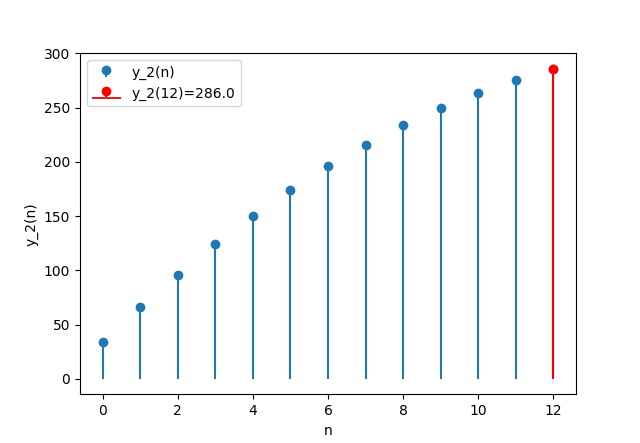
\includegraphics[width=\columnwidth]{graph_2}
\caption{$y_2\brak{n}$ vs n }
\label{graph:ee25-g3}
\end{figure}

 
\item
-5 + -8 + -11 ... -230


\begin{align}
x_3\brak{n} &= \brak{x_3\brak{0} -3n}u_{\brak{n}}\\
\implies -230 &= -5 -3n \\
\implies n &= 75
\end{align}
\begin{enumerate}
\item
Z-Transform of $x_3\brak{n}$ :
Using $\eqref{eq:ztrans}$
\begin{align}
X_3\brak{z} &=  \frac{-5z}{\brak{z-1}^{1}} -
       \frac{3z}{\brak{z-1}^{2}} \label{eq:ee25-8}
,\quad \abs {z}>\abs{1} 
\end{align}

    
\item
Z-Transform of $y_3\brak{n}$ :
\begin{align}
    y_3\brak{n} &= x_3\brak{n} * h\brak{n} \\
         h\brak{n} &= u\brak{n} \\
    Y_3\brak{z} &= X_3\brak{z} * H\brak{z}\\
             &= \brak{\frac{-5z}{{\brak{z-1}^1}}-
       \frac{3z}{\brak{z-1}^2}}\brak{\frac{z}{z-1}}
,\quad \abs {z}>\abs{1} 
    \end{align}

    \item
Inversion of $Y_3\brak{z}$ :
Using Contour Integration :
\begin{align}
y_1(75)&=\frac{1}{2\pi j}\oint_{C}Y(z) \;z^{74} \;dz\\  
    \implies &=\frac{1}{2\pi j}\oint_{C}\brak{\frac{-5z^{76}}{\brak{z-1}^2}-
       \frac{3z^{76}}{\brak{z-1}^3}} \;dz 
\end{align}
Using \eqref{eq:ee25-r}
For $R_1$ , $m=2$ :
\begin{align}
    R_1 &=\frac{1}{\brak {1}!}\lim\limits_{z\to 1}\frac{d}{dz}\brak {{(z-1)}^{2}\frac{-5z^{76}}{{(z-1)}^2}}   \\
    &=-5\lim\limits_{z\to 1}\frac{d}{dz}(z^{76})   \\
    &= -380
        \end{align}
  For $R_2$ , $m=3$ :
    \begin{align}
    R_2 &=\frac{1}{\brak {2}!}\lim\limits_{z\to 1}\frac{d^{2}}{dz^{2}}\brak {{(z-1)}^{3}\frac{3z^{76}}{{(z-1)}^3}}   \\
    &=1.5\lim\limits_{z\to 1}\frac{d^2}{dz^2}(z^{76})   \\
    &= -8550\\
    R_1 + R_2 &= -8930\\
    \implies  y_3{(75)} &= -8930
\end{align}
    \end{enumerate}



\begin{figure}[ht!]   
\centering
    \graphicspath{ {ncert-maths/10/5/3/2/figs/} }
    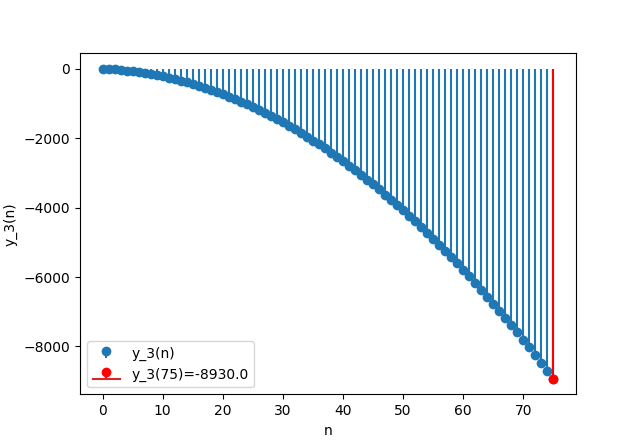
\includegraphics[width=\columnwidth]{graph_3}
    \caption{$y_3\brak{n}$ vs n }
    \label{graph:ee25-g4}
\end{figure}
 \end{enumerate}
 %\end{document}

\pagebreak
\item Show that $a_0$ , $a_1$ , $a_2$
, . . ., $a_n$
, . . . form an AP where an is defined as below :
\begin{enumerate}
    \item $a_n$ = $(3 + 4n)$ 
    \item $a_n$ = $(9 - 5n)$ 
\end{enumerate}
Also find the sum of the first 15 terms in each case.
\solution
\iffalse
\let\negmedspace\undefined
\let\negthickspace\undefined
\documentclass[journal,12pt,twocolumn]{IEEEtran}
\usepackage{cite}
\usepackage{amsmath,amssymb,amsfonts,amsthm}
\usepackage{algorithmic}
\usepackage{graphicx}
\usepackage{textcomp}
\usepackage{xcolor}
\usepackage{txfonts}
\usepackage{listings}
\usepackage{enumitem}
\usepackage{mathtools}
\usepackage{gensymb}
\usepackage{comment}
\usepackage[breaklinks=true]{hyperref}
\usepackage{tkz-euclide} 
\usepackage{listings}
\usepackage{gvv}                                        
\def\inputGnumericTable{}                                 
\usepackage[latin1]{inputenc}                                
\usepackage{color}                                            
\usepackage{array}                                            
\usepackage{longtable}                                       
\usepackage{calc}                                             
\usepackage{multirow}                                         
\usepackage{hhline}                                           
\usepackage{ifthen}                                           
\usepackage{lscape}
\usepackage{amsmath}
\usepackage{caption}
\newtheorem{theorem}{Theorem}[section]
\newtheorem{problem}{Problem}
\newtheorem{proposition}{Proposition}[section]
\newtheorem{lemma}{Lemma}[section]
\newtheorem{corollary}[theorem]{Corollary}
\newtheorem{example}{Example}[section]
\newtheorem{definition}[problem]{Definition}
\newcommand{\BEQA}{\begin{eqnarray}}
\newcommand{\EEQA}{\end{eqnarray}}
\newcommand{\define}{\stackrel{\triangle}{=}}
\theoremstyle{remark}
\newtheorem{rem}{Remark}
\begin{document}

\bibliographystyle{IEEEtran}
\vspace{3cm}

\title{NCERT 10.5.3 10Q}
\author{EE22BTECH11010 - Venkatesh D Bandawar $^{*}$% <-this % stops a space
}
\maketitle
\newpage
\bigskip

\renewcommand{\thefigure}{\theenumi}
\renewcommand{\thetable}{\theenumi}

\textbf{Question:} Show that $a_0$ , $a_1$ , $a_2$
, . . ., $a_n$
, . . . form an AP where an is defined as below :
\begin{enumerate}
    \item $a_n$ = $(3 + 4n)$ 
    \item $a_n$ = $(9 - 5n)$ 
\end{enumerate}
Also find the sum of the first 15 terms in each case.

\textbf{Solution:} 
\fi
    \begin{table}[!h] 
    \centering
    \begin{tabular}{|c|c|c|}
\hline
     \textbf{Parameter} & \textbf{Description} & \textbf{Value} \\
     \hline
     \multirow{3}{*}{$x_i(n)$} & \multirow{3}{*}{$i^{th}$Discrete signal} & $(3+4n)u(n)$\\
     \cline{3-3}
     & & $(9-5n)u(n)$\\
     \hline
     \multirow{3}{*}{$x_i(0)$} & \multirow{3}{*}{First term of $i^{th}$AP} & $3$ \\
     \cline{3-3}
     & & $9$\\
     \hline
     \multirow{3}{*}{$d_i$} & \multirow{3}{*}{common difference of $i^{th}$AP} & $4$ \\
     \cline{3-3}
     & & $-5$\\
     \hline
\end{tabular}

    \caption{Given parameters}
    \label{given parameters list}
    \end{table}
\begin{enumerate} 
    \item From equation \eqref{eq:APSum}
    \begin{align}
        X(z) &= \frac{3}{1-z^{-1}} + \frac{4.z^{-1}}{(1-z^{-1})^2} ; |z|>1\\
        \because y(n) &= x(n) * u(n)\\
        Y(z) &= X(z)U(z)\\
        &= \sbrak{\frac{3}{\brak{1-z^{-1}}^2} + \frac{4 z^{-1}}{\brak{1-z^{-1}}^3}} 
    \end{align}
    Using contour integration for inverse Z transformation,
    \begin{align}
        y(14) &= \frac{1}{2\pi j}\int Y(z) z^{13} dz \\
         &= \frac{1}{2\pi j}\int \frac{3.z^{15}}{(z-1)^{2}} dz + \frac{1}{2\pi j}\int \frac{4.z^{15}}{(z-1)^{3}} dz\\
        \because R&=\frac{1}{\brak {m-1}!}\lim\limits_{z\to a}\frac{d^{m-1}}{dz^{m-1}}\brak {{(z-a)}^{m}f\brak z}\\
        R_1 &=\frac{1}{1!}\lim\limits_{z\to 1}\frac{d}{dz}\brak {(z-1)^2.\frac{3.z^{15}}{(z-1)^{2}}}\\
        &= 45\\
        R_2 &=\frac{1}{2!}\lim\limits_{z\to 1}\frac{d^2}{dz^2}\brak {(z-1)^3.\frac{4.z^{15}}{(z-1)^{3}}}\\
        &= 420\\
        \implies y(14) &= R_1 + R_2 \\
        &= 465
    \end{align}
    
    \begin{figure}[!h] 
    \centering
    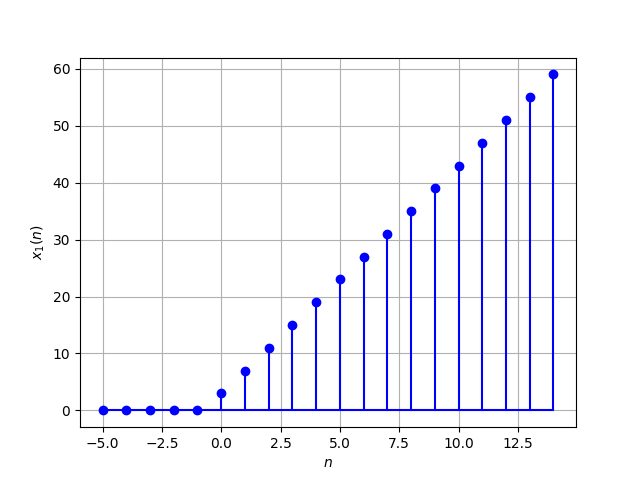
\includegraphics[width=\columnwidth]{ncert-maths/10/5/3/10/figs/signal_x1.png}
    \caption{$x_1(n)=(3+4n)u(n)$}
    \label{fig:Graph1_math.10.5.3.10}
    \end{figure}

    \begin{figure}[!h] 
    \centering
    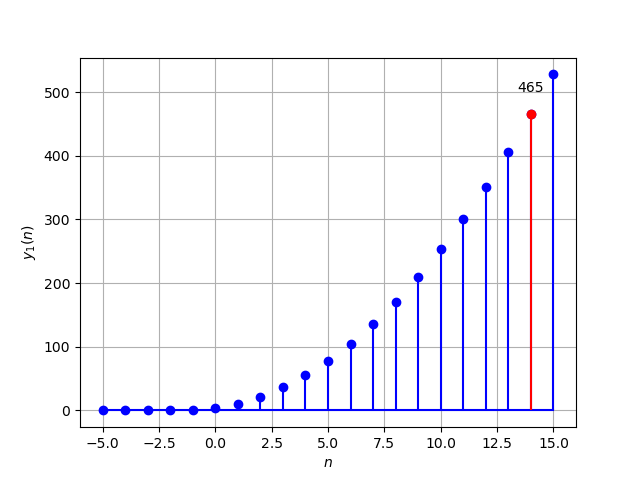
\includegraphics[width=\columnwidth]{ncert-maths/10/5/3/10/figs/signal_y1.png}
    \caption{$x_1(n)=(2n^2+5n+3)u(n)$}
    \label{fig:Graph2_math.10.5.3.10}
    \end{figure}
    
    \item From equation  \eqref{eq:APSum}
    \begin{align}
         X(z) &= \frac{9}{1-z^{-1}} - \frac{5.z^{-1}}{(1-z^{-1})^2} ; |z|>1\\
        \because y(n) &= x(n) * u(n)\\
        Y(z) &= X(z)U(z)\\
         &= \sbrak{\frac{9}{\brak{1-z^{-1}}^2} - \frac{5 z^{-1}}{\brak{1-z^{-1}}^3}}
    \end{align}
    Using contour integration for inverse Z transformation,
    \begin{align}
       y(14) &= \frac{1}{2\pi j}\int Y(z) z^{13} dz \\
         &= \frac{1}{2\pi j}\int \frac{9.z^{15}}{(z-1)^{2}} dz - \frac{1}{2\pi j}\int \frac{5.z^{15}}{(z-1)^{3}} dz\\
        \because R&=\frac{1}{\brak {m-1}!}\lim\limits_{z\to a}\frac{d^{m-1}}{dz^{m-1}}\brak {{(z-a)}^{m}f\brak z}\\
        R_1 &=\frac{1}{1!}\lim\limits_{z\to 1}\frac{d}{dz}\brak {(z-1)^2.\frac{9.z^{15}}{(z-1)^{2}}}\\
         &= 135\\
        R_2 &=\frac{1}{2!}\lim\limits_{z\to 1}\frac{d^2}{dz^2}\brak {(z-1)^3.\frac{5.z^{15}}{(z-1)^{3}}}\\
         &= 525\\
        \implies y(14) &= R_1 - R_2 \\
        &= -390
    \end{align}
    
    \begin{figure}[!h] 
    \centering
    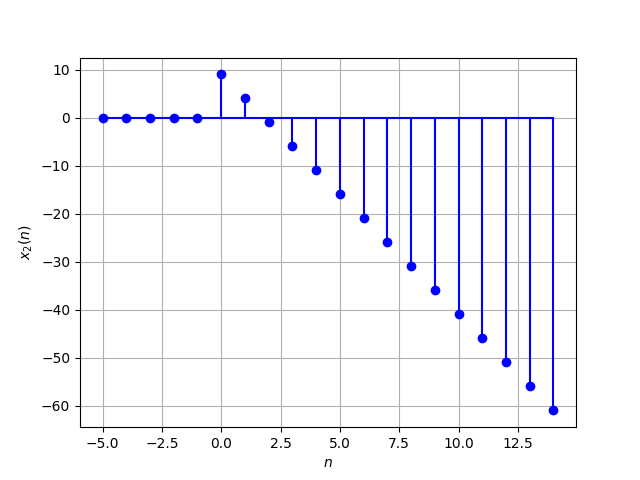
\includegraphics[width=\columnwidth]{ncert-maths/10/5/3/10/figs/signal_x2.png}
    \caption{$x_2(n)=(9-5n)u(n)$}
    \label{fig:Graph3_math.10.5.3.10}
    \end{figure}

    \begin{figure}[!h] 
    \centering
    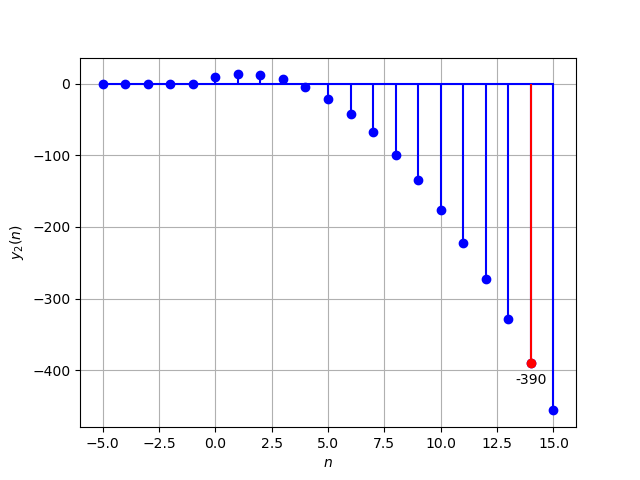
\includegraphics[width=\columnwidth]{ncert-maths/10/5/3/10/figs/signal_y2.png}
    \caption{$x_2(n)=(-5n^2+13n+18)u(n)$}
    \label{fig:Graph4_math.10.5.3.10}
    \end{figure}

\end{enumerate} 


\pagebreak
\item If the sum of $n$ terms of an AP is $(pn + qn^2)$, where $p$ and $q$ are constants, find the common difference.
\solution
		\iffalse
\let\negmedspace\undefined
\let\negthickspace\undefined
\documentclass[journal,12pt,twocolumn]{IEEEtran}
\usepackage{cite}
\usepackage{amsmath,amssymb,amsfonts,amsthm}
\usepackage{algorithmic}
\usepackage{graphicx}
\usepackage{textcomp}
\usepackage{xcolor}
\usepackage{txfonts}
\usepackage{listings}
\usepackage{enumitem}
\usepackage{mathtools}
\usepackage{gensymb}
\usepackage{comment}
\usepackage[breaklinks=true]{hyperref}
\usepackage{tkz-euclide} 
\usepackage{listings}
\usepackage{gvv}                                        
\def\inputGnumericTable{}                                
\usepackage[latin1]{inputenc}                            
\usepackage{color}                                       
\usepackage{array}                                       
\usepackage{longtable}                                   
\usepackage{calc}                              
\usepackage{tikz}
\usepackage{multirow}                                    
\usepackage{hhline}                                      
\usepackage{ifthen}                            
\usepackage{caption}
\usepackage{lscape}
\usepackage{amsmath}
\newtheorem{theorem}{Theorem}[section]
\newtheorem{problem}{Problem}
\newtheorem{proposition}{Proposition}[section]
\newtheorem{lemma}{Lemma}[section]
\newtheorem{corollary}[theorem]{Corollary}
\newtheorem{example}{Example}[section]
\newtheorem{definition}[problem]{Definition}
\newcommand{\BEQA}{\begin{eqnarray}}
\newcommand{\EEQA}{\end{eqnarray}}
\newcommand{\define}{\stackrel{\triangle}{=}}
\theoremstyle{remark}
\newtheorem{rem}{Remark}

\begin{document}

\bibliographystyle{IEEEtran}
\vspace{3cm}

\title{NCERT Math 11.9.2 Q8}
\author{EE23BTECH11009 - AROSHISH PRADHAN$^{*}$% <-this % stops a space
}
\maketitle
\newpage
\bigskip
\textbf{Question:} If the sum of $n$ terms of an AP is $(pn + qn^2)$, where $p$ and $q$ are constants, find the common difference.

\solution
\fi
\begin{table}[!h]
    \centering
    \begin{tabular}{|c|c|c|}
    \hline
      \textbf{Symbol}   &  \textbf{Value} & \textbf{Description}\\
    \hline
       $y(n)$  & $(pn + qn^2)$ & Sum of $n$ terms\\
    \hline
        $x(n)$ &  & $n^{th}$ term of AP\\
    \hline
        $d$ & $x(n+1) - x(n)$ &Common Difference\\
    \hline 
\end{tabular}

    \caption{Given Parameters}
    \label{tab:1_Math.11.9.2.8}
\end{table}

Sum of $n$ terms, as a discrete signal:
\begin{align}
    y(n) = (pn + qn^2)u(n) \label{eq:1_Math.11.9.2.8}
\end{align}
Taking the $Z$-Transform,
\begin{enumerate}
    \item $\mathcal{Z}\{u(n)\}$
\begin{align}
    u(n) \system{Z} \frac{1}{1-z^{-1}} \{\abs{z} > 1\} \label{eq:2_Math.11.9.2.8}
\end{align}
    \item $\mathcal{Z}\{nu(n)\}$
\begin{align}
    nu(n) \system{Z} \frac{z^{-1}}{(1-z^{-1})^2}\, \{\abs{z} > 1\} \label{eq:3_Math.11.9.2.8}
\end{align}
\item $\mathcal{Z}{\{n^2 u(n)\}}$
    \begin{align}
        n^2u(n) \system{Z} \frac{z^{-1}(1+z^{-1})}{(1-z^{-1})^3}\, \{\abs{z} > 1\} \label{eq:4_Math.11.9.2.8}
    \end{align}
\end{enumerate}
Taking the Z-Transform of \eqref{eq:1_Math.11.9.2.8} using \eqref{eq:3_Math.11.9.2.8} and \eqref{eq:4_Math.11.9.2.8}
\begin{align}
      Y(z) = p\brak{\frac{z^{-1}}{(1-z^{-1})^2}} + q\brak{\frac{z^{-1}(1 + z^{-1})}{(1-z^{-1})^3}}
\end{align}
Now, 
\begin{align}
    y(n) &= x(n) \ast u(n)\\
    \implies Y(z) &= X(z)U(z)\\
    \implies X(z) &= \frac{Y(z)}{U(z)}\label{eq:8_Math.11.9.2.8}
\end{align}
Using \eqref{eq:2_Math.11.9.2.8} in \eqref{eq:8_Math.11.9.2.8},
\begin{align}
    X(z) &= p\brak{\frac{z^{-1}}{(1-z^{-1})}} + q\brak{\frac{z^{-1}(1 + z^{-1})}{(1-z^{-1})^2}}
\end{align}
Using contour integration for inverse Z-Transform:
\begin{align}
    x(n) &= \frac{1}{2\pi j} \oint_C X(z) z^{n-1}dz\\
    &= \frac{1}{2 \pi j} \oint_C  \sbrak{p\brak{\frac{z^{-1}}{(1-z^{-1})}} + q\brak{\frac{z^{-1}(1 + z^{-1})}{(1-z^{-1})^2}}}z^{n-1}dz
\end{align}
Calculating the residues $R_1$ and $R_2$ at pole $z=1$:
\begin{align}
    R_1 &= \frac{1}{0!} \lim_{z \to 1}(z-1)\brak{p\brak{\frac{z^{-1}}{1-z^{-1}}}}z^{n-1}\\
    &= p\\
    R_2 &= \frac{1}{1!} \lim_{z \to 1}\frac{d}{dz}\brak{(z-1)^2q\brak{\frac{z^{-1}(1 + z^{-1})}{(1-z^{-1})^2}}}z^{n-1}\\
    &= q\lim_{z \to 1}\frac{d}{dz}\brak{z^{n} + z^{n-1}}\\
    &= q(2n-1)\\
    \implies x(n) &= R_1 + R_2\\
    &= p + q(2n-1)
\end{align}
Writing x(n) as a discrete signal we get:
\begin{align}
    x(n) &= (p-q)u(n) + 2qnu(n)\label{eq:19_Math.11.9.2.8}
\end{align}
To simplify, use $n=0$:
\begin{align}
    y(0)&=x(0)\\
    \implies 0 &= (p-q)u(0) +2q(0)u(0)\\
    \implies p &= q
\end{align}
$\therefore$ \eqref{eq:19_Math.11.9.2.8} an be written as:
\begin{align}
    x(n) &= 2qnu(n)
\end{align}
Common difference is given by:
\begin{align}
    d &= x(n+1) - x(n)\\
    &= 2q
\end{align}
\begin{figure}[!h]
    \centering
    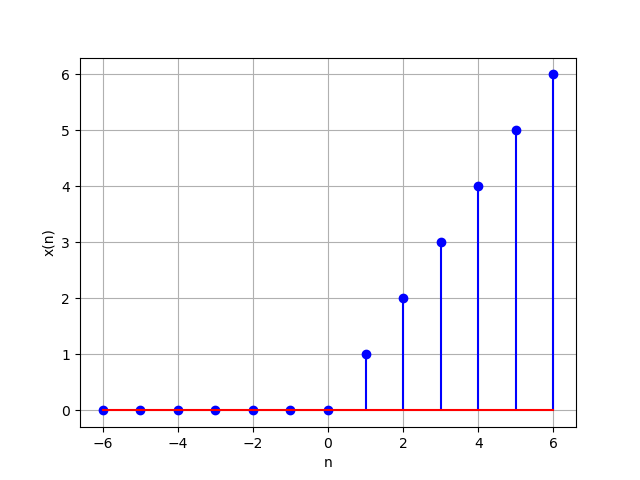
\includegraphics[width = \columnwidth]{ncert-maths/11/9/2/8/figs/x_plot.png}
    \caption{Plot of x(n) vs n for $p=q=0.5$}
    \label{fig:1_Math.11.9.2.8}
\end{figure}
\begin{figure}[!h]
    \centering
    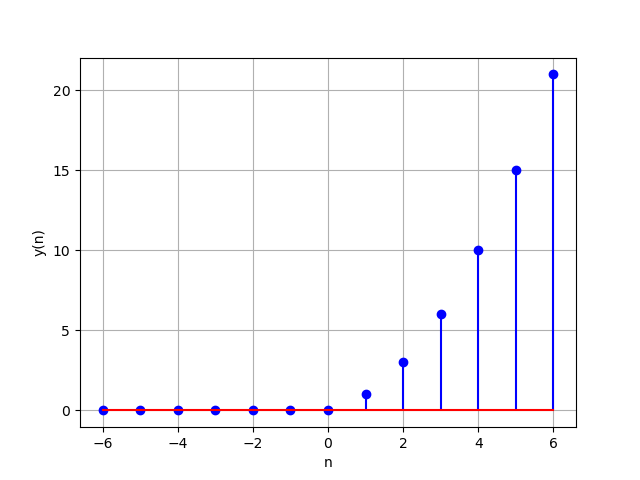
\includegraphics[width = \columnwidth]{ncert-maths/11/9/2/8/figs/y_plot.png}
    \caption{Plot of y(n) vs n for $p=q=0.5$}
    \label{fig:2_Math.11.9.2.8}
\end{figure}


\pagebreak
\item Find the sum of the first 40 positive integers divisible by 6\\
	\solution
		\iffalse
\let\negmedspace\undefined
\let\negthickspace\undefined
\documentclass[journal,12pt,twocolumn]{IEEEtran}
\usepackage{cite}
\usepackage{amsmath,amssymb,amsfonts,amsthm}
\usepackage{algorithmic}
\usepackage{graphicx}
\usepackage{textcomp}
\usepackage{xcolor}
\usepackage{txfonts}
\usepackage{listings}
\usepackage{enumitem}
\usepackage{mathtools}
\usepackage{gensymb}
\usepackage[breaklinks=true]{hyperref}
\usepackage{tkz-euclide} % loads  TikZ and tkz-base
\usepackage{listings}
\usepackage{gvv}
%
%\usepackage{setspace}
%\usepackage{gensymb}
%\doublespacing
%\singlespacing

%\usepackage{graphicx}
%\usepackage{amssymb}
%\usepackage{relsize}
%\usepackage[cmex10]{amsmath}
%\usepackage{amsthm}
%\interdisplaylinepenalty=2500
%\savesymbol{iint}
%\usepackage{txfonts}
%\restoresymbol{TXF}{iint}
%\usepackage{wasysym}
%\usepackage{amsthm}
%\usepackage{iithtlc}
%\usepackage{mathrsfs}
%\usepackage{txfonts}
%\usepackage{stfloats}
%\usepackage{bm}
%\usepackage{cite}
%\usepackage{cases}
%\usepackage{subfig}
%\usepackage{xtab}
%\usepackage{longtable}
%\usepackage{multirow}
%\usepackage{algorithm}
%\usepackage{algpseudocode}
%\usepackage{enumitem}
%\usepackage{mathtools}
%\usepackage{tikz}
%\usepackage{circuitikz}
%\usepackage{verbatim}
%\usepackage{tfrupee}
%\usepackage{stmaryrd}
%\usetkzobj{all}
%    \usepackage{color}                                            %%
%    \usepackage{array}                                            %%
%    \usepackage{longtable}                                        %%
%    \usepackage{calc}                                             %%
%    \usepackage{multirow}                                         %%
%    \usepackage{hhline}                                           %%
%    \usepackage{ifthen}                                           %%
  %optionally \brak{for landscape tables embedded in another document}: %%
%    \usepackage{lscape}     
%\usepackage{multicol}
%\usepackage{chngcntr}
%\usepackage{enumerate}

%\usepackage{wasysym}
%\documentclass[conference]{IEEEtran}
%\IEEEoverridecommandlockouts
% The preceding line is only needed to identify funding in the first footnote. If that is unneeded, please comment it out.

\newtheorem{theorem}{Theorem}[section]
\newtheorem{problem}{Problem}
\newtheorem{proposition}{Proposition}[section]
\newtheorem{lemma}{Lemma}[section]
\newtheorem{corollary}[theorem]{Corollary}
\newtheorem{example}{Example}[section]
\newtheorem{definition}[problem]{Definition}
%\newtheorem{thm}{Theorem}[section] 
%\newtheorem{defn}[thm]{Definition}
%\newtheorem{algorithm}{Algorithm}[section]
%\newtheorem{cor}{Corollary}
\newcommand{\BEQA}{\begin{eqnarray}}
\newcommand{\EEQA}{\end{eqnarray}}
\newcommand{\define}{\stackrel{\triangle}{=}}
\theoremstyle{remark}
\newtheorem{rem}{Remark}

%\bibliographystyle{ieeetr}
\begin{document}
%

\bibliographystyle{IEEEtran}


\vspace{3cm}

\title{
%  \logo{
Assignment-1 

\large{EE:1205 \brak{Signals  Systems}}

Indian Institute of Technology, Hyderabad
%  }
}
\author{Md Ayaan Ashraf

EE23BTECH11041
}  
%\title{
%  \logo{Matrix Analysis through Octave}{\begin{center}\includegraphics[scale=.24]{tlc}\end{center}}{}{HAMDSP}
%}


% paper title
% can use linebreaks \\ within to get better formatting as desired
%\title{Matrix Analysis through Octave}
%
%
% author names and IEEE memberships
% note positions of commas and nonbreaking spaces \brak{ ~ } LaTeX will not break
% a structure at a ~ so this keeps an author's name from being broken across
% two lines.
% use \thanks{} to gain access to the first footnote area
% a separate \thanks must be used for each paragraph as LaTeX2e's \thanks
% was not built to handle multiple paragraphs
%
%\author{<-this % stops a space
%\thanks{}}
%}
% note the % following the last \IEEEmembership and also \thanks - 
% these prevent an unwanted space from occurring between the last author name
% and the end of the author line. i.e., if you had this:
% 
% \author{....lastname \thanks{...} \thanks{...} }
%                     ^------------^------------^----Do not want these spaces!
%
% a space would be appended to the last name and could cause every name on that
% line to be shifted left slightly. This is one of those "LaTeX things". For
% instance, "\textbf{A} \textbf{B}" will typeset as "A B" not "AB". To get
% "AB" then you have to do: "\textbf{A}\textbf{B}"
% \thanks is no different in this regard, so shield the last } of each \thanks
% that ends a line with a % and do not let a space in before the next \thanks.
% Spaces after \IEEEmembership other than the last one are OK \brak{and needed} as
% you are supposed to have spaces between the names. For what it is worth,
% this is a minor point as most people would not even notice if the said evil
% space somehow managed to creep in.



% The paper headers
%\markboth{Journal of \LaTeX\ Class Files,~Vol.~6, No.~1, January~2007}%
%{Shell \MakeLowercase{\textit{et al.}}: Bare Demo of IEEEtran.cls for Journals}
% The only time the second header will appear is for the odd numbered pages
% after the title page when using the twoside option.
% 
% *** Note that you probably will NOT want to include the author's ***
% *** name in the headers of peer review papers.                   ***
% You can use \ifCLASSOPTIONpeerreview for conditional compilation here if
% you desire.




% If you want to put a publisher's ID mark on the page you can do it like
% this:
%\IEEEpubid{0000--0000/00\$00.00~\copyright~2007 IEEE}
% Remember, if you use this you must call \IEEEpubidadjcol in the second
% column for its text to clear the IEEEpubid mark.



% make the title area
\maketitle

\newpage

%\tableofcontents

\bigskip
 
\renewcommand{\thefigure}{\theenumi}
\renewcommand{\thetable}{\theenumi}
%\renewcommand{\theequation}{\theenumi}
\section*{\textit{\textbf{Question 10.5.3.12:}}}
 Find the sum of the first 40 positive integers divisible by 6.
\section*{\textit{\textbf{Solution:}}}
\fi

\begin{table}[ht]
  \centering
  \begin{tabular}{|c||c||c|}
    \hline
    Parameter & Description & Value \\
    \hline
     x(0) & First Term & 6\\
     \hline
     d & Common Difference & 6\\
    \hline
  \end{tabular}
  \vspace{2mm}
  \caption{Parameter Table 10.5.3.12}
\end{table}


\begin{align}
x\brak{n}= &\brak{6+6n}\brak{u\brak{n}}\\
\implies X\brak{z}= &\frac6{1-z^{-1}} + \frac{6z^{-1}}{\brak{1-z^{-1}}^{2}} \quad\eqref{eq:APSum}\\
\implies X\brak{z}=& \frac6{{\brak{1-z^{-1}}}^2} ,\quad |z|>1\\
y\brak{n}=& x\brak{n}* u\brak{n}\\
\implies Y\brak{z}=& X\brak{z}U\brak{z} \\
=& \frac{6}{\brak{1-z^{-1}}^{3}}, \quad |z|>1
\end{align}
Using contour integration to find the inverse Z-transform:\\
\begin{align}
    \implies y\brak{39}=&\dfrac{1}{2\pi j}\oint_{C}Y\brak{z} \;z^{38} \;dz\\
    =&\dfrac{1}{2\pi j}\oint_{C}\dfrac{6z^{41}}{\brak{{z-1}}^{3}} \;dz 
\end{align}
We can observe that there is only a three times repeated pole at z=1,
\begin{align}
    \implies R&=\dfrac{1}{\brak {m-1}!}\lim\limits_{z\to a}\dfrac{d^{m-1}}{dz^{m-1}}\brak {{\brak{z-a}}^{m}f\brak z}  
\end{align}
\begin{align}
    &=\dfrac{1}{\brak {2}!}\lim\limits_{z\to 1}\dfrac{d^{2}}{dz^{2}}\brak {{\brak{z-1}}^{3}\dfrac{6z^{41}}{{\brak{z-1}}^3}}   \\
    &=3\lim\limits_{z\to 1}\dfrac{d^2}{dz^2}\brak{z^{41}}\\
    &=4920
\end{align}
\begin{align}
    \therefore \boxed{y\brak{39}=4920}
\end{align}
\begin{figure}[ht]
    \centering
    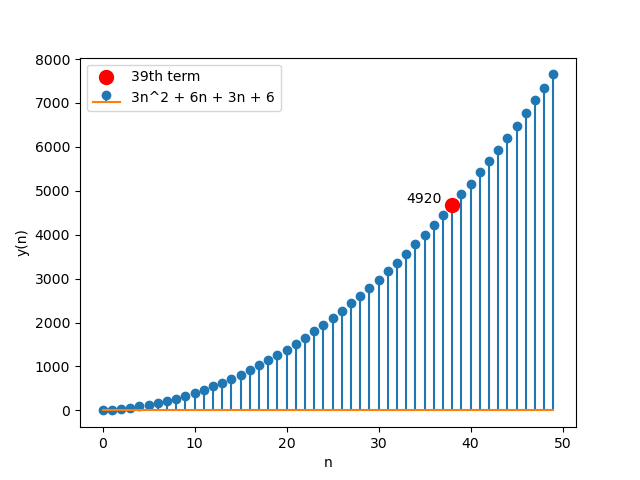
\includegraphics[width=\columnwidth]{ncert-maths/10/5/3/12/figs/fig1.png}
    \caption{Plot of y\brak{n} $vs$ n}
    \label{fig: 10.5.3.12}
\end{figure}


\pagebreak
\item If the sum of certain number of terms in a AP 25,22,19,... is 116. Find the last term.\\
\solution
\iffalse
\let\negmedspace\undefined
\let\negthickspace\undefined
\documentclass[journal,12pt,twocolumn]{IEEEtran}
\usepackage{cite}
\usepackage{amsmath,amssymb,amsfonts,amsthm}
\usepackage{algorithmic}
\usepackage{graphicx}
\usepackage{textcomp}
\usepackage{xcolor}
\usepackage{txfonts}
\usepackage{listings}
\usepackage{enumitem}
\usepackage{mathtools}
\usepackage{gensymb}
\usepackage{comment}
\usepackage[breaklinks=true]{hyperref}
\usepackage{tkz-euclide}
\usepackage{listings}
\usepackage{gvv}
\def\inputGnumericTable{}
\usepackage[latin1]{inputenc}
\usepackage{color}
\usepackage{array}
\usepackage{longtable}
\usepackage{calc}
\usepackage{multirow}
\usepackage{hhline}
\usepackage{ifthen}
\usepackage{lscape}

\newtheorem{theorem}{Theorem}[section]
\newtheorem{problem}{Problem}
\newtheorem{proposition}{Proposition}[section]
\newtheorem{lemma}{Lemma}[section]
\newtheorem{corollary}[theorem]{Corollary}
\newtheorem{example}{Example}[section]
\newtheorem{definition}[problem]{Definition}
\newcommand{\BEQA}{\begin{eqnarray}}
\newcommand{\EEQA}{\end{eqnarray}}
\newcommand{\define}{\stackrel{\triangle}{=}}
\theoremstyle{remark}
\newtheorem{rem}{Remark}
\begin{document}

\bibliographystyle{IEEEtran}
\vspace{3cm}

\title{NCERT Discrete - 11.9.2.6}
\author{EE23BTECH11212 - Manugunta Meghana Sai$^{*}$% <-this % stops a space
}
\maketitle
\newpage
\bigskip

\renewcommand{\thefigure}{\theenumi}
\renewcommand{\thetable}{\theenumi}

\vspace{3cm}
\textbf{NCERT Maths 11.9.2 Q6} 
If the sum of certain number of terms in a AP 25,22,19,... is 116. Find the last term.\\
\solution
\fi
\begin{table}[h!]
    \centering
    \begin{tabular}{|c|c|c|}
	\hline
	\textbf{Symbol} & \textbf{Value} & \textbf{Description} \\[6pt]
	\hline
	$x(0)$ & $25$ & first term of AP \\[6pt]
	\hline
	$d$ & $-3$ & common difference \\[6pt]
	\hline
	$x(n)$ & $(25-3n)u(n)$ & $n$-th term of AP \\[6pt]
	\hline
	$y(n)$ & $116$ & sum of terms \\[6pt]
	\hline 
\end{tabular}

    \caption{Input Parameters}
    \label{tab:table1}
\end{table}
\begin{align}
	x(n) = (25 - 3n)u(n)
	\label{eq:11.9.2.6}
\end{align}
Applying Z transform:
\begin{align}
    x(z) &=\frac{25}{1-z^{-1}} - \frac{3z^{-1}}{(1-z^{-1})^2}\\
    &= \frac{25-28z^{-1}}{(1-z^{-1})^2} 
\end{align}
     Region of Convergence or R.O.C :
\begin{align}
     \abs{z}>1
\end{align}
For AP, the sum of first n+1 terms can be written as :
\begin{align}
	 y(n)&=x(n)*u(n)
\end{align}  
Applying Z transform on both sides
\begin{align}
	Y(z) &= X(z)U(z)\\
	&=\frac{25}{(1-z^{-1})^2} - \frac{3z^{-1}}{(1-z^{-1})^3}
\end{align}
Using contour integration to find inverse Z transform:
\begin{align}
	y(n) &= \frac{1}{2\pi j} \oint_C Y(z) z^{n-1} dz\\
	&= \frac{1}{2\pi j} \oint_C \left[ \frac{25}{(1-z^{-1})^2} - \frac{3z^{-1}}{(1-z^{-1})^3} \right]z^{n-1} \, dz
\end{align}
The sum of the terms of the sequence is computed using the residue theorem, expressed as $R_i$, which represents the residue of the Z-transform at $ z=1 $ for the expression $ Y(z) $.
\begin{align}
	R_i=R_1 + R_2
\end{align}
 $R_1$ and $R_2$ are residues calculated at the poles of the Z-transform.
\begin{align}
		R_1 &= \frac{1}{{(2-1)!}} \left. \frac{d (25z^{n+1})}{dz} \right|_{z=1} \\
	&=25(n+1)
\end{align}
\begin{align}
	R_2 &= \frac{1}{{(3-1)!}} \left. \frac{d^2(-3z^{n+1})}{dz^2} \right|_{z=1} \\
	&= \frac{-3}{2}(n+1)(n)
\end{align}
The sum of terms is given by $R_i$:
 \begin{align}
25(n+1)	+ \frac{-3}{2} n(n+1) = 116 
 \end{align}
Solving the equation gives :
\begin{align}
	n&=7\\ n&=8.667
\end{align}
Since n can take only integer values, $n=8.667$ is rejected. 
Upon substituting the value of n in equation~\eqref{eq:11.9.2.6}:
\begin{align}
	x(7)=4
\end{align}
Hence the last term of the given AP is 4.
\begin{figure}[h!]
    \centering
    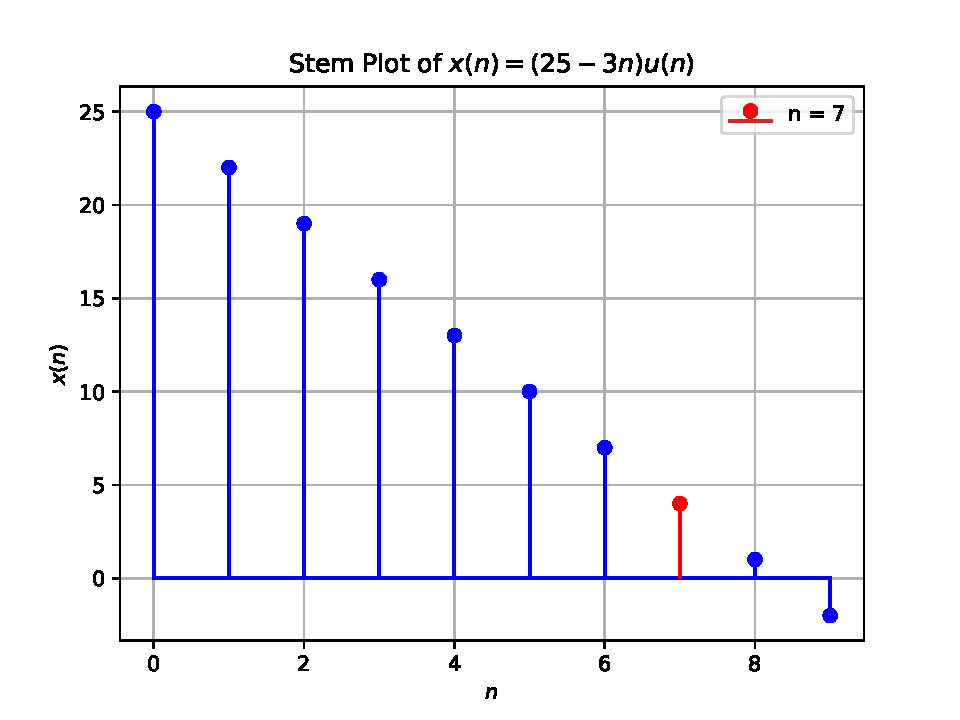
\includegraphics[width=\columnwidth]{ncert-maths/11/9/2/6/figs/stem_plot.pdf}
\end{figure}
%\end{document}

\pagebreak

\item The first and the last terms of an AP are 17 and 350 respectively. If the common difference
is 9, how many terms are there and what is their sum?\\
\solution 
\iffalse
\let\negmedspace\undefined
\let\negthickspace\undefined
\documentclass[journal,12pt,twocolumn]{IEEEtran}
\usepackage{cite}
\usepackage{amsmath,amssymb,amsfonts,amsthm}
\usepackage{algorithmic}
\usepackage{graphicx}
\usepackage{textcomp}
\usepackage{xcolor}
\usepackage{txfonts}
\usepackage{listings}
\usepackage{enumitem}
\usepackage{mathtools}
\usepackage{gensymb}
\usepackage{comment}
\usepackage[breaklinks=true]{hyperref}
\usepackage{tkz-euclide} 
\usepackage{listings}
\usepackage{gvv}                                        
\def\inputGnumericTable{}                                 
\usepackage[latin1]{inputenc}                                
\usepackage{color}                                            
\usepackage{array}                                            
\usepackage{longtable}                                       
\usepackage{calc}                                             
\usepackage{multirow}                                         
\usepackage{hhline}                                           
\usepackage{ifthen}                                           
\usepackage{lscape}

\newtheorem{theorem}{Theorem}[section]
\newtheorem{problem}{Problem}
\newtheorem{proposition}{Proposition}[section]
\newtheorem{lemma}{Lemma}[section]
\newtheorem{corollary}[theorem]{Corollary}
\newtheorem{example}{Example}[section]
\newtheorem{definition}[problem]{Definition}
\newcommand{\BEQA}{\begin{eqnarray}}
\newcommand{\EEQA}{\end{eqnarray}}
\newcommand{\define}{\stackrel{\triangle}{=}}
\theoremstyle{remark}
\newtheorem{rem}{Remark}
\begin{document}
\bibliographystyle{IEEEtran}
\vspace{3cm}
\title{10.5.3}
\author{EE23BTECH11027 - K RAHUL$^{*}$% <-this % stops a space
}
\maketitle
\newpage
\bigskip
\renewcommand{\thefigure}{\theenumi}
\renewcommand{\thetable}{\theenumi}
QUESTION:\\
The first and the last terms of an AP are 17 and 350 respectively. If the common difference
is 9, how many terms are there and what is their sum?\\
\bigskip \bigskip


SOLUTION:
\fi
\begin{table}[ht]
\setlength{\arrayrulewidth}{0.3mm}
\setlength{\tabcolsep}{15pt}
\renewcommand{\arraystretch}{1.5}



\begin{tabular}{ |p{1cm}|p{3cm}|p{1cm}| }
\hline
\multicolumn{3}{|c|}{Parameters in expression}\\
\hline
Symbol & Description & Value\\
\hline
$x(n)$ & $n^{th}$ term of series & \\
\hline
$x(l)$ & Last($l^{th}$) term of series & 350\\
\hline
$x(0)$ & Starting ($0^{th}$) term of series & 17 \\
\hline
d & Common difference of AP & 9\\
\hline
\end{tabular}
\caption{Parameters}
 %Table 1: Parameters



\end{table}
\begin{align}
x(n) &= (x(0) + nd)u(n)\\
x(l)&=(17+9l)u(l)
\end{align}

Thus,
\begin{align}{l = 37}\end{align}
Using \eqref{eq:APSum},
\begin{align}
	X(z) &= \frac{(17-8z^{-1})}{{(1-z^{-1})}^2},
\quad \abs{z} > \abs{1}\\
y(n) &= x(n) * u(n)\\
\implies Y(z) &= X(z)U(z)\\
&= \frac{(17-8z^{-1})}{(1-z^{-1})^{3}}\end{align}
\bigskip
Using contour integral to find Z transform, we get
\begin{align}
    y(37) &= \frac{1}{2\pi j} \oint _C Y(z)z^{36}dz\\
    &= \frac{1}{2\pi j} \oint _C \frac{(17-8z^{-1})}{(1-z^{-1})^{3}}z^{36}dz
\end{align}
Now, using Cauchy's residual theorem and observing the fact that 3 repeated poles exist at z = 1, 
\begin{align}
    R &= \frac{1}{(k-1)!}\lim_{z \to c}\frac{d^{k-1}}{dz^{k-1}}((z-c)^kf(z))\\
    &= \frac{1}{2!}\lim_{z \to 1}\frac{d^{k-1}}{dz^{k-1}}((z-1)^3\frac{(17-8z^{-1})}{(1-z^{-1})^{3}}z^{36})\\
    &=\frac{1}{2}\lim_{z \to 1}\frac{d^2}{dz^2}(17z^{39} - 8z^{38})\\
    &= 6973
\end{align}
\begin{figure}[h]
    %\caption{Stem Plot of $x(n)$ v/s n}
    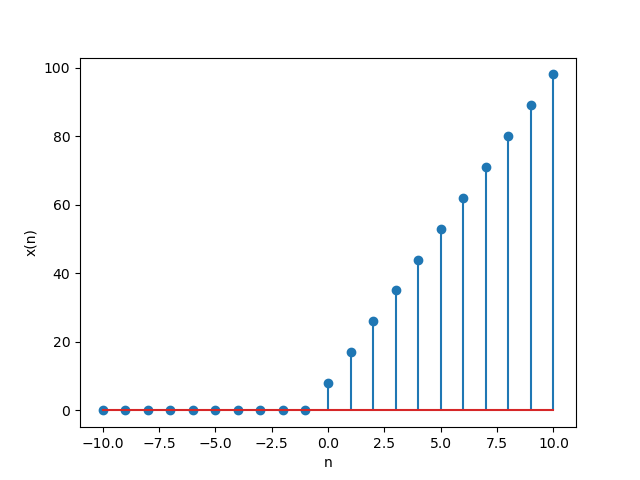
\includegraphics[width=0.5\textwidth]{ncert-maths/10/5/3/6/figs/x(n)_plot.png}\label{fig:stem-plot}
    \caption{Stem Plot of $x(n)$ v/s n}
\end{figure}
%\end{document}

\pagebreak
\item A small terrace at a football ground comprises of 15 steps each of which is 50
m long and built of solid concrete.Each step has a rise of 1/4 m and a tread of
1/2 m. Calculate the total volume of concrete required to build the terrace.
[Hint: Volume of concrete required to build the first step=\begin{align}
    V&=\frac{1}{4} \cdot \frac{1}{2} \cdot 50 
\end{align}\\
\solution 
\iffalse
\let\negmedspace\undefined
\let\negthickspace\undefined
\documentclass[journal,12pt,twocolumn]{IEEEtran}
\usepackage{cite}
\usepackage{amsmath,amssymb,amsfonts,amsthm}
\usepackage{algorithmic}
\usepackage{graphicx}
\usepackage{textcomp}
\usepackage{xcolor}
\usepackage{txfonts}
\usepackage{listings}
\usepackage{enumitem}
\usepackage{mathtools}
\usepackage{gensymb}
\usepackage{comment}
\usepackage[breaklinks=true]{hyperref}
\usepackage{tkz-euclide} 
\usepackage{listings}
\usepackage{gvv}                                        
\def\inputGnumericTable{}                                 
\usepackage[latin1]{inputenc}                                
\usepackage{color}                                            
\usepackage{array}                                            
\usepackage{longtable}                                       
\usepackage{calc}                                             
\usepackage{multirow}                                         
\usepackage{hhline}                                           
\usepackage{ifthen}                                           
\usepackage{lscape}

\newtheorem{theorem}{Theorem}[section]
\newtheorem{problem}{Problem}
\newtheorem{proposition}{Proposition}[section]
\newtheorem{lemma}{Lemma}[section]
\newtheorem{corollary}[theorem]{Corollary}
\newtheorem{example}{Example}[section]
\newtheorem{definition}[problem]{Definition}
\newcommand{\BEQA}{\begin{eqnarray}}
\newcommand{\EEQA}{\end{eqnarray}}
\newcommand{\define}{\stackrel{\triangle}{=}}
\theoremstyle{remark}
\newtheorem{rem}{Remark}
\begin{document}

\bibliographystyle{IEEEtran}
\vspace{3cm}

\title{10.5.4-5}
\author{EE23BTECH11033-killana jaswanth}
\maketitle
\newpage

\bigskip

\renewcommand{\thefigure}{\theenumi}
\renewcommand{\thetable}{\theenumi}
Question:\\
A small terrace at a football ground comprises of 15 steps each of which is 50
m long and built of solid concrete.Each step has a rise of 1/4 m and a tread of
1/2 m. Calculate the total volume of concrete required to build the terrace.
[Hint: Volume of concrete required to build the first step=\begin{align}
    V&=\frac{1}{4} \cdot \frac{1}{2} \cdot 50 
\end{align}
solution:
\fi
here\begin{table}[!ht]
 \centering
  \begin{tabular}{|c|c|c|}
\hline
\textbf{parameter}& \textbf{description}& \textbf{value}
\\\hline
\multirow{3}{1em}\\$x\brak{0}$&first term&$6.25$
\\\hline
$d$&common difference&$6.25$
\\\hline
$n$&no of terms $-1$&$14$
\\\hline
$x\brak{n}$&volume of \brak{n+1}th step&$\brak{6.25+6.25n}u\brak{n}$
\\\hline
\end{tabular}


   \caption{formula parameters}
   \label{tab:10.5.4.5}
   \end{table}
\begin{align}
 X\brak{z}&=\frac{x(0)}{1-\,z^{-1}}+\frac{dz^{-1}}{\brak{1-{z^{-1}}}^2}\:\:
\quad\abs{z}>\abs{1}\\
\implies X(z)&=\brak{\frac{6.25}{\brak{1-z^{-1}}^2}} \quad\abs{z}>\abs{1}
\end{align}
\begin{figure}[!ht]
    \centering
    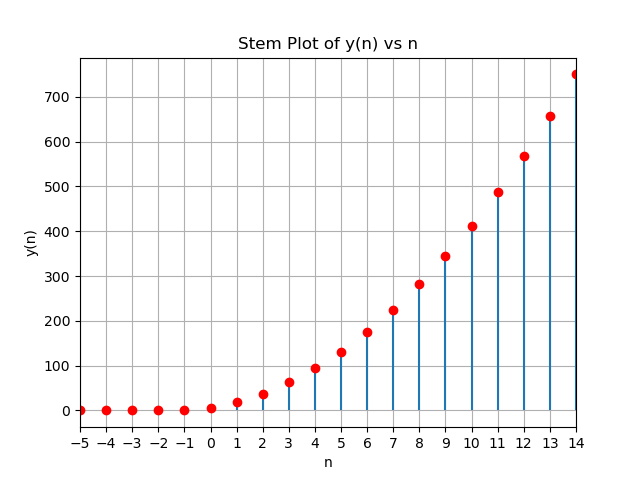
\includegraphics[width=1\linewidth]{ncert-maths/10/5/4/5/figs/fig.png}
    \caption{plot y\brak{n} vs n}
    \label{fig:enter-label}
\end{figure}
\begin{align}
y\brak{n}&=x\brak{n}*u\brak{n}\\
\implies Y\brak{z}&=X\brak{z}U\brak{z}\\
U\brak{z}&=\frac{1}{1-\,z^{-1}}\quad\abs{z}>\abs{1}\\
Y\brak{z}&=\brak{\frac{6.25}{1-\,z^{-1}}+\frac{6.25z^{-1}}{\brak{1-{z^{-1}}}^2}}\brak{\frac{1}{1-\,z^{-1}}}\quad\abs{z}>\abs{1}\\
Y\brak{z}&=\frac{6.25z^3}{\brak{z-1}^{3}} \quad\abs{z}>\abs{1}
\end{align}
  contour integration to find inverse z transform
\begin{align}
y(14)&=\frac{1}{2{\pi}j}{\oint_c}Y\brak{z}z^{13}dz\\
&=\frac{1}{2{\pi}j}{\oint_c}{\frac{6.25z^{16}}{\brak{z-1}^{3}}}
\end{align}
pole at 1 repeated 3 times\\
\begin{align}
\implies m&=3\\
R&=\frac{1}{\brak{m-1}!}\lim_{z\to a}\frac{d^{m-1}}{dz^{m-1}}\brak{\brak{z-a}^mf{\brak{z}}}\\
\implies y(14)&=\frac{1}{\brak{2!}}\lim_{z\to 1}\frac{d^2}{dz^2}\brak{\brak{z-1}^{3}\frac{6.25z^{16}}{\brak{z-1}^3}}\\
&=3.125\lim_{z\to1}\frac{d^2}{dz^2}\brak{z^{16}}\\
y\brak{14}&=750
\end{align}

\pagebreak

\item Given a GP with a = 729 and $7^{th}$ term 64, find $S_7$.\\
\solution 
\iffalse
\let\negmedspace\undefined
\let\negthickspace\undefined
\documentclass[journal,12pt,twocolumn]{IEEEtran}
\usepackage{cite}
\usepackage{amsmath,amssymb,amsfonts,amsthm}
\usepackage{algorithmic}
\usepackage{graphicx}
\usepackage{textcomp}
\usepackage{xcolor}
\usepackage{txfonts}
\usepackage{listings}
\usepackage{enumitem}
\usepackage{mathtools}
\usepackage{gensymb}
\usepackage{comment}
\usepackage[breaklinks=true]{hyperref}
\usepackage{tkz-euclide} 
\usepackage{listings}
\usepackage{gvv}                                        
\def\inputGnumericTable{}                                 
\usepackage[latin1]{inputenc}                                
\usepackage{color}                                            
\usepackage{array}                                            
\usepackage{longtable}                                       
\usepackage{calc}                                             
\usepackage{multirow}                                         
\usepackage{hhline}                                           
\usepackage{ifthen}                                           
\usepackage{lscape}

\newtheorem{theorem}{Theorem}[section]
\newtheorem{problem}{Problem}
\newtheorem{proposition}{Proposition}[section]
\newtheorem{lemma}{Lemma}[section]
\newtheorem{corollary}[theorem]{Corollary}
\newtheorem{example}{Example}[section]
\newtheorem{definition}[problem]{Definition}
\newcommand{\BEQA}{\begin{eqnarray}}
\newcommand{\EEQA}{\end{eqnarray}}
\newcommand{\define}{\stackrel{\triangle}{=}}
\theoremstyle{remark}
\newtheorem{rem}{Remark}

\graphicspath{{./figs/}}

\begin{document}

\bibliographystyle{IEEEtran}
\vspace{3cm}

\Large\title{NCERT Question 11.9.3.15}
\large\author{EE23BTECH11032 - Kaustubh Parag Khachane $^{*}$% <-this % stops a space
}
\maketitle
\newpage
\bigskip

\renewcommand{\thefigure}{\theenumi}
\renewcommand{\thetable}{\theenumi}
\large\textbf{Question 11.9.3.15} :

Given a GP with a = 729 and $7^{th}$ term 64, find $S_7$.

\solution
\fi
\begin{table}[ht] 
\centering
\setlength{\extrarowheight}{8pt}
\begin{tabular}{|l|l|l|}
    \hline
    \textbf{Parameter} & \textbf{Description} & \textbf{Value} \\
    \hline
     x\brak{0} & First Term & 729 \\
    \hline
     r & Common Ratio & \\
    \hline
      x\brak{n} & $\brak{n+1}^{th}$ Term & $x\brak{0}r^{n}u\brak{n}$ \\
    \hline
     x\brak{6} & $7^{th}$ Term & 64 \\
    \hline
    y\brak{k} & Sum of first \brak{k+1} terms & \\
    \hline
  \end{tabular}
  \vspace{4mm}
 \caption{Parameter Table}
 \label{tab:table0_11_9_3_15}
\end{table}


from \tabref{tab:table0_11_9_3_15} :
\begin{align}
    &x\brak{6} = x\brak{0}r^6\\
    \implies &64 = 729r^6\\
    &\therefore r = \frac{2}{3}\label{eq:eq2_11_9_3_15}
\end{align}
%using equation \eqref{eq:eq1} and equation \eqref{eq:eq2}
%\begin{align}
% s\brak{6} &= 729\frac{\brak{\frac{2}{3}}^6 - 1}{\frac{2}{3} - 1}\\
% & = \frac{729\left(\frac{2187 - 128}{2187}\right)}{\frac{1}{3}}\\
%\implies s\brak{6} &= 2059
%\end{align}
using \tabref{tab:table0_11_9_3_15} and equation \eqref{eq:eq2_11_9_3_15}
\begin{align}
    &X\brak{z} = \frac{729}{1 - \frac{2}{3}z^{-1}}\label{eq:eq6_11_9_3_15},\abs{z} > \frac{2}{3}
\end{align}
using \tabref{tab:table0_11_9_3_15} and equation \eqref{eq:eq6_11_9_3_15}
\begin{align}
    Y\brak{z} &= \frac{729}{\brak{1 - \frac{2}{3}z^{-1}}\brak{1-z^{-1}}}\\
    &= 2187\brak{\frac{1}{1-z^{-1}} - \frac{\frac{2}{3}}{1 - \frac{2}{3}z^{-1}}} \label{eq:eq5_11_9_3_15},\abs{z}  > 1
\end{align}
Using contour integration for inverse z transform,
\begin{align}
    y\brak{6} &= \frac{1}{2\pi j}\oint Y\brak{z} z^{5} dz \label{eq:eq12_11_9_3_15}
\end{align}
Using equation \eqref{eq:eq5_11_9_3_15} in \eqref{eq:eq12_11_9_3_15} :
\begin{align}
    y\brak{6}= \frac{1}{2\pi j}\brak{\oint\frac{2187z^{6}}{z-1}dz - \oint\frac{1458z^{6}}{z - \frac{2}{3}} dz} \label{eq:eq8_11_9_3_15}
\end{align}
\begin{align}
    \frac{1}{2\pi j}\brak{\oint\frac{2187z^{6}}{z - 1}dz} &= 2187\label{eq:eq9_11_9_3_15}\\
     \frac{1}{2\pi j}\brak{\oint\frac{1458z^{6}}{z - \frac{2}{3}}dz}  &= 128\label{eq:eq10_11_9_3_15}
     \end{align}
using equations \eqref{eq:eq9_11_9_3_15} and \eqref{eq:eq10_11_9_3_15} in \eqref{eq:eq8_11_9_3_15}:
\begin{align}
y\brak{6} &= 2187 - 128\\
&= 2059
\end{align}

\begin{figure}[!ht]
\centering
\begin{center}
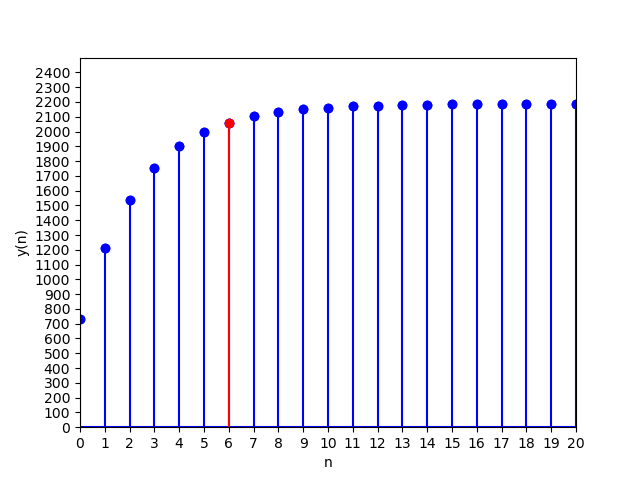
\includegraphics[width=\columnwidth]{ncert-maths/11/9/3/15/figs/Figure_1.png}
\end{center}
\caption{Plot of $y\brak{n}$}
\end{figure}
\begin{figure}[!ht]
\centering
\begin{center}
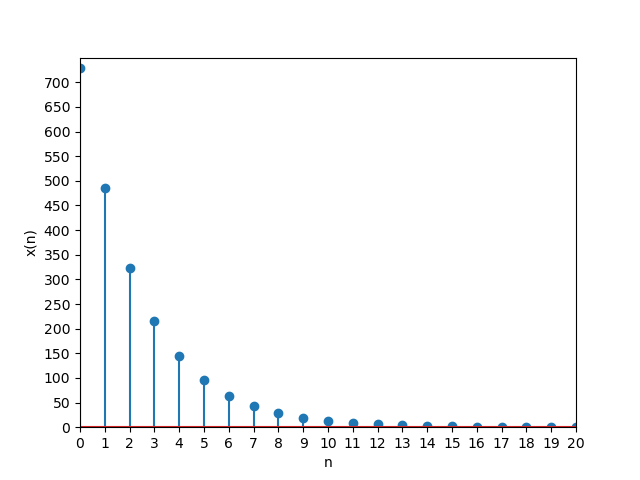
\includegraphics[width=\columnwidth]{ncert-maths/11/9/3/15/figs/Figure_2.png}
\end{center}
\caption{Plot of $x\brak{n}$}
\end{figure}

\pagebreak

\item Find the sum of all natural numbers lying between 100 and 1000, which are
multiples of 5.\\
\solution
\iffalse
\let\negmedspace\undefined
\let\negthickspace\undefined
\documentclass[journal,12pt,twocolumn]{IEEEtran}
\usepackage{cite}
\usepackage{amsmath,amssymb,amsfonts,amsthm}
\usepackage{algorithmic}
\usepackage{graphicx}
\usepackage{textcomp}
\usepackage{xcolor}
\usepackage{txfonts}
\usepackage{listings}
\usepackage{enumitem}
\usepackage{mathtools}
\usepackage{gensymb}
\usepackage{comment}
\usepackage[breaklinks=true]{hyperref}
\usepackage{tkz-euclide} 
\usepackage{listings}
\usepackage{gvv}

\def\inputGnumericTable{}                                
\usepackage[latin1]{inputenc}                 
\usepackage{color}                            
\usepackage{array}                            
\usepackage{longtable}                        
\usepackage{calc}                            
\usepackage{multirow}                      
\usepackage{hhline}                           
\usepackage{ifthen}                          
\usepackage{lscape}
\usepackage{amsmath}
\newtheorem{theorem}{Theorem}[section]
\newtheorem{problem}{Problem}
\newtheorem{proposition}{Proposition}[section]
\newtheorem{lemma}{Lemma}[section]
\newtheorem{corollary}[theorem]{Corollary}
\newtheorem{example}{Example}[section]
\newtheorem{definition}[problem]{Definition}
\newcommand{\BEQA}{\begin{eqnarray}}
\newcommand{\EEQA}{\end{eqnarray}}
\newcommand{\define}{\stackrel{\triangle}{=}}
\theoremstyle{remark}
\newtheorem{rem}{Remark}


\begin{document}
%

\bibliographystyle{IEEEtran}


\vspace{3cm}

\title{
%	\logo{
Discrete 11.9.2 

\large{EE:1205 Signals and System}

Indian Institute of Technology, Hyderabad
%	}
}
\author{Prashant Maurya

EE23BTECH11218
\maketitle

\newpage

%\tableofcontents

\bigskip

\renewcommand{\thefigure}{\arabic{figure}}
\renewcommand{\thetable}{\arabic{table}}
\flushleft{\textbf{Question-2 :} Find the sum of all natural numbers lying between 100 and 1000, which are
multiples of 5.}\\
\bigskip
\textbf{Solution:}
\fi
\begin{table}[!h]
	\centering
	\begin{tabular}{|c|c|c|}
    \hline
     Parameter & Description & Value \\
    \hline
     $x(0)$ & First Term & 105\\
     \hline
     $d$ & Common Difference & 5\\
    \hline
    $n$ & Total terms & 179 \\ 
    \hline
    $x(178)$ & Last Term & 995\\
    \hline
    $m$ & No of poles & 3\\
    \hline
\end{tabular}

	\vspace{6 pt}
	\caption{Given Parameters}
\end{table}
\begin{align}
	x\brak{n}= & \brak{105+5n}\brak{u(n)}
\end{align}
On taking Z transform
\begin{align}
X\brak{z}= &\frac {x\brak{0}} {\brak{1-z^{-1}}} + \frac {dz^{-1}} {\brak{1-z^{-1}}^2} \\
= &\dfrac{105}{1-z^{-1}} + \frac{5z^{-1}}{\brak{1-z^{-1}}^{2}}\\
\implies X\brak{z}=& \dfrac{105-100z^{-1}}{{\brak{1-z^{-1}}}^2} \quad |z|>1\\
y\brak{n}=& x\brak{n}* u\brak{n}\\
\implies Y\brak{z}=& X\brak{z}U\brak{z}\\
=& \dfrac{105-100z^{-1}}{{(1-z^{-1})}^2}\frac1 {\brak{1-z^{-1}}} \\
=& \dfrac{105-100z^{-1}}{\brak{1-z^{-1}}^{3}} \quad |z|>1
\end{align}
Using contour integration to find the inverse Z-transform:\\
\begin{align}
    \implies y\brak{178}=&\dfrac{1}{2\pi j}\oint_{C}Y\brak{z} \;z^{177} \;dz\\
    =&\dfrac{1}{2\pi j}\oint_{C}\dfrac{\brak{105-100z^{-1}}{z^{177}}}{\brak{{1-z^{-1}}}^{3}} \;dz 
\end{align}
We can observe that there is only a 3 times repeated pole at $z=1$,
\begin{align}
    \implies R&=\dfrac{1}{\brak {m-1}!}\lim\limits_{z\to a}\dfrac{d^{m-1}}{dz^{m-1}}\brak {{\brak{z-a}}^{m}f\brak z}  
\end{align}
\begin{align}
    &=\dfrac{1}{\brak {2}!}\lim\limits_{z\to 1}\dfrac{d^{2}}{dz^{2}}\brak {{\brak{z-1}}^{3}\dfrac{\brak{105-100z^{-1}}z^{180}}{{\brak{z-1}}^3}}\\
    &=\dfrac{1}{2}{\lim\limits_{z\to 1}\dfrac{d^2}{dz^2}\brak{105z^{180}-100z^{179}}}\\
     &=98450
\end{align}
\begin{align}
    \therefore y\brak{178}=98450
\end{align}
\begin{figure}[ht]
    \centering
    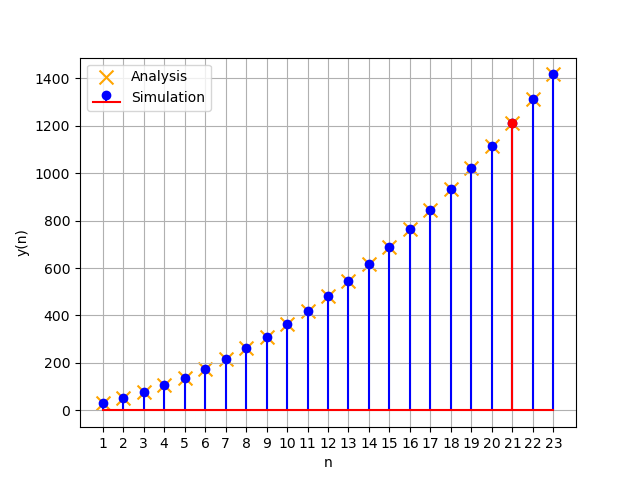
\includegraphics[width=\columnwidth]{ncert-maths/11/9/2/2/figures/fig1.png}
    \caption{Plot of $x(n)$ $vs$ $n$}
\end{figure}
%\end{document}

\pagebreak

\item Find the sum of odd numbers between 0 and 50.\\
\solution
\input{}
\pagebreak

\end{enumerate}
